\documentclass{report}

\usepackage[utf8]{inputenc} % Charakter-Kodierung
\usepackage[german]{babel} % Sprache

\usepackage[table,xcdraw]{xcolor} % Tabellen Farben
\usepackage{tabularx} % Dynamische Tabellenbreite
\usepackage{tcolorbox} % Graue Boxen
\usepackage{hyperref} % url Umgebung
\usepackage{todonotes} % Notizen
\usepackage{natbib} % Bibliographie
\usepackage{fancyhdr} % Header und Footer
\usepackage{multirow} % Multizeile
\usepackage{geometry} % Page layout
\usepackage{color} % Text Farben
\usepackage{longtable} % Longtable
\usepackage{float} % Damit die Abbildungen auch an der richtigen Position bleiben.

% Page layout
\geometry{
	bottom=3.5cm,
	headheight=180pt
}

% Nummerierung der ersten Seiten verhindern
\pagenumbering{gobble}

% Bibstyle
\bibliographystyle{plain}

% Header / Footer
\fancypagestyle{plain}{
	\fancyhf{}% Clear header/footer
	\fancyhead[R]{
\includegraphics[width=4cm]{img/cau-logo-2017}} % Rechter header
	\fancyhead[L]{\leftmark} % Linker header
	\fancyfoot[R]{\thepage} % Rechter footer
	\fancyfoot[L]{
\includegraphics[width=1cm]{img/se-logo}} % Linker footer	
}
\pagestyle{plain}

\renewcommand{\headrulewidth}{0.5pt} % Unnötige Informationen der Kapitelangabe
\renewcommand{\footrulewidth}{0.2pt} % entfernen
\renewcommand{\chaptermark}[1]{\markboth{{#1}}{}}




% Zahlen für Fußnoten
\renewcommand{\thefootnote}{\arabic{footnote}}
\renewcommand{\thempfootnote}{\arabic{mpfootnote}}

%%%%% Ausfüllen %%%%%

% Gruppenname
\newcommand{\gruppenname}{Gruppe LMS2 UE1}

% Projektname
\newcommand{\projektname}{Smart Building Solutions}

% Semester
\newcommand{\semester}{Sommer 2021}



% Titelseite

\title{
	\vspace*{-3cm}
	Entwurfsdokumentation\\
	\projektname\\
	-\\
	\color{gray}
	Softwareprojekt \semester\\
	\gruppenname\\
	\vspace*{5mm}
	
\includegraphics[width=\textwidth]{img/logo}
}

\author{
	\begin{tabular}{r l@{\hspace{8\tabcolsep}} r} 
		Eddy & Wu & \multirow{8}{*}{ 
\includegraphics{img/se-logo} } \\
		Julius & Daum \\
		Lea Marie & Sch\"umann \\
		Luca Anthony & Schwarz \\
		Natalie & Kaufhold \\
		Philipp & Wieck \\
		Till & Kurzenberger \\
		Yilmaz Atakan & Kara \\
	\end{tabular}
}

\date{\today}





% Dokument

\begin{document}
	\maketitle
	
	%%%% Bitte löschen oder auskommentieren %%%%
	%%%%%%%%% Dient nur als Hilfe %%%%%%%%%%
	
%	\chapter*{Tipps und Hilfen}\label{chp:tipps}
%	\vspace*{-1.4cm}
%	\begin{tcolorbox}
%		\textbf{Information:} Dieses Kapitel und alle folgenden grauen Boxen dienen als Hilfestellungen und sollen im fertigen Dokument nicht enthalten sein. 
%		%
%		\\\\
%		%
%		Zur Versionsverwaltung während des Softwareprojekts muss \textit{Git} genutzt werden.
%		Git führt Textdokumente mit unterschiedlichen Zeilenbearbeitungen automatisch zusammen.
%		Wir empfehlen den Einsatz von \LaTeX~für alle Textdokumente.
%		Um das Auto-Merging zu unterstützen, sollte nach jedem Satzende eine neue Zeile im Quelltext begonnen werden.
%		Die .tex-Datei dieser PDF verdeutlicht dies.
%		Erkennt Git, dass eine gleiche Zeile bearbeitet wurde, wird ein Konflikt auftreten.
%		Dieser kann in der entsprechenden Datei von Hand mittels eines Texteditors behoben werden.
%		%
%		\\\\
%		%
%		Fußnoten\footnote{\url{https://www.se.informatik.uni-kiel.de/en}} werden für Homepages genutzt.
%		Zitierungen können mittels eines \textit{cite}-Befehls gesetzt, z.B. \textit{citep}~\citep{Shaw2003WritingGoodSoftwareEngineeringesearchPapersMinitutorial}.
%		%
%		\\\\
%		%
%		Tipps zur UML-Modellierung können im SE-Wiki\footnote{\url{https://git.informatik.uni-kiel.de/ag-se/teaching-public/wikis/home}} nachgelesen werden.
%		Achtet darauf, dass eure Diagramme stets lesbar (Vektor-Grafiken!) und gut strukturiert sind.
%		Oftmals ist es sinnvoll ein bis zwei Sätze zusätzlich für Diagrammelemente zu formulieren.
%		So können Missverständnisse ausgeschlossen werden, was einen Einfluss auf die Korrektur haben kann.
%		Diagramme für unwichtige Tätigkeiten (z.B. Login / Logout, User erstellen / löschen, Passwort ändern etc.) sind nicht erforderlich.
%		Achtet weiterhin darauf, dass interne Abläufe und Methodenaufrufe in den Frameworks nicht modelliert werden sollen.
%		So soll z.B. das Sequenzdiagramm für das Erstellen einer Rechnung nicht interne Methoden und Abläufe des benutzten Frameworks abbilden, sondern nur diese Operationen zeigen, die Teil eures zukünftigen Codes sind.
%	\end{tcolorbox}
%	
%	\todo[inline]{So kann eine TODO-Notiz erzeugt werden}
%	
%	\begin{figure}[h]
%		\centering
%		\missingfigure{So kann eine Placeholder-Grafik beispielsweise in den Text eingefügt werden.}		
%		\caption{Beschreibung}
%		\label{fig:x}
%	\end{figure}
		
	%%%%%%%%%%%%%%%%%%%%%%%%%%%%%%
	
	\tableofcontents 
	
	\chapter{Einleitung}\label{chp:einleitung}
	\pagenumbering{arabic} % Nummerierung starten
	\thispagestyle{fancy}
	\section{Dokumentaufbau}\label{sec:dokumentaufbau}
\begin{tcolorbox}
    Inhalt und Struktur des vorliegenden Dokuments skizzieren (Fließtext).
\end{tcolorbox}

\section{Zweckbestimmung}\label{sec:zweckbestimmung}
\textbf{Smart Building Solutions} hat als Ziel die entwickelte Software f\"ur Auftragnehmer und Auftraggeber im Baugewerbe zur Verf\"ugung zu stellen.  Die Software verwendet die vom Unternehmen bereitgestellten Vertrags- und Projektdaten,  um den Status einzelner Projektbestandteile geeignet und den Anforderungen des Nutzers entsprechend in Form von Diagrammen und Statusbalken zu visualisieren. \\
Dabei soll f\"ur Mitarbeiter einzelner Organisationen eine Web-Oberfl\"ache zur Verf\"ugung stehen.  F\"ur  Mitarbeiter,  welche konkret am Bauprozess einzelner Leistungspositionen beteiligt sind,  ist eine Oberfl\"ache in Form einer mobilen Applikation bereitgestellt.  Die mobile Anwendung verf\"ugt dann \"uber ausgew\"ahlte Funktionalit\"aten zur R\"uckmeldung und Visualisierung von Baufortschritt,  sowie Status\"anderung der einzelnen Leistungspositionen.  \"Anderungen an diesen Daten werden entsprechend mit der Webanwendung synchronisiert.  Sie ist ausgelegt f\"ur die Nutzung auf einem geeigneten Endger\"at unter Verwendung von Android 6 oder h\"oher.  Die Weboberfl\"ache hingegen bietet im Webbrowser,  bspw. Chrome oder Firefox, volle Funktionalit\"at zur Darstellung und Erstellung von Diagrammen nach benutzerspezifischen Kriterien, die M\"oglichkeit Nutzer zu registrieren,  Projekt- und Vertragsdaten einzusehen und den Status einzelner Leistungspositionen anzupassen. \\
Ein Systemadministrator, vom jeweiligen Bauunternehmen selbst ernannt,  erh\"alt die entsprechenden Rechte  einen Mitarbeiter als Organisations-Administrator auszuw\"ahlen.
Zugriffsm\"oglichkeiten auf die einzelnen Funktionen von Webanwendung und mobiler Applikation sind entsprechend abh\"angig von der Position oder Benutzerrolle eines Mitarbeiters im konkreten Unternehmen und werden von einem zum Organisations-Administrator beauftragten Mitarbeiter des Unternehmens selbstst\"andig vergeben.  Die Registrierung einzelner Nutzer wird ebenfalls von diesem Mitarbeiter durchgef\"uhrt.

\newpage
\section{Entwicklungsumgebung}\label{sec:entwicklungsumgebung}

\centering
\begin{longtable}[h]{p{4cm} p{2cm} p{8cm}}
    \caption{Enwicklungsumgebung - Web-Oberfl\"ache und Backend}
    \label{table:entwicklungsumgebung}
    \endlastfoot
    \multicolumn{3}{r}{{Weitergeführt auf der folgenden Seite}}                                                                                            \\
    \endfoot
    \endhead
    \rowcolor[HTML]{C0C0C0}
    \textbf{Software}                & \textbf{Version} & \textbf{URL}                                                                                     \\
    Eclipse                          & neueste          & \url{https://www.eclipse.org/}                                                                   \\
    \rowcolor[HTML]{E7E7E7}
    IntelliJ IDEA                    & neueste          & \url{https://www.jetbrains.com/de-de/idea/}                                                      \\
    VSCode                           & neueste          & \url{https://code.visualstudio.com/}                                                             \\
    \rowcolor[HTML]{E7E7E7}
    Java Development Kit             & 11.0.11          & \url{https://www.oracle.com/de/java/technologies/javase-jdk11-downloads.html}                    \\
    Gradle                           & 7.1.1            & \url{https://gradle.org/releases/}                                                               \\
    \rowcolor[HTML]{E7E7E7}
    Spring Boot                      & 2.5.4            & \url{https://mvnrepository.com/artifact/org.springframework.boot/spring-boot/2.5.4}              \\
    Spring Dependency Management     & 1.0.11           & \url{https://plugins.gradle.org/plugin/io.spring.dependency-management}                          \\
    \rowcolor[HTML]{E7E7E7}
    Spring Boot Starter Data JPA     & neueste          & \url{https://mvnrepository.com/artifact/org.springframework.boot/spring-boot-starter-data-jpa}   \\
    Spring Boot Starter Validation   & neueste          & \url{https://mvnrepository.com/artifact/org.springframework.boot/spring-boot-starter-validation} \\
    \rowcolor[HTML]{E7E7E7}
    Spring Boot Starter Security     & neueste          & \url{https://mvnrepository.com/artifact/org.springframework.boot/spring-boot-starter-security}   \\
    Spring Boot Starter Thymeleaf    & neueste          & \url{https://mvnrepository.com/artifact/org.springframework.boot/spring-boot-starter-thymeleaf}  \\
    \rowcolor[HTML]{E7E7E7}
    Spring Boot Starter Web          & neueste          & \url{https://mvnrepository.com/artifact/org.springframework.boot/spring-boot-starter-web}        \\
    Thymeleaf Extras Springsecurity5 & neueste          & \url{https://mvnrepository.com/artifact/org.thymeleaf.extras/thymeleaf-extras-springsecurity5}   \\
    \rowcolor[HTML]{E7E7E7}
    Spring Boot Devtools             & neueste          & \url{https://mvnrepository.com/artifact/org.springframework.boot/spring-boot-devtools}           \\
    H2 Database                      & neueste          & \url{https://mvnrepository.com/artifact/com.h2database/h2}                                       \\
    \rowcolor[HTML]{E7E7E7}
    Spring Boot Starter Test         & neueste          & \url{https://mvnrepository.com/artifact/org.springframework.boot/spring-boot-starter-test}       \\
    Spring Security Test             & neueste          & \url{https://mvnrepository.com/artifact/org.springframework.security/spring-security-test}       \\
    \rowcolor[HTML]{E7E7E7}
    JUnit Jupiter API                & 5.7.2            & \url{https://mvnrepository.com/artifact/org.junit.jupiter/junit-jupiter-api}                     \\
    Bootstrap                        & neueste(5.1.0)   & \url{https://getbootstrap.com/docs/5.1/getting-started/download/}                                \\
\end{longtable}

\begin{longtable}[h]{p{4cm} p{2cm} p{8cm}}
    \caption{Enwicklungsumgebung - mobile Applikation}
    \label{table:entwicklungsumgebung}
    \endlastfoot
    \multicolumn{3}{r}{{Weitergeführt auf der folgenden Seite}} \\
    \endfoot
    \endhead
    \rowcolor[HTML]{C0C0C0}
    \textbf{Software}    & \textbf{Version} & \textbf{URL} \\
    Java Development Kit & 11.0.11          & \url{https://www.oracle.com/de/java/technologies/javase-jdk11-downloads.html} \\
    \rowcolor[HTML]{E7E7E7}
    Android Studio           & neueste        & \url{https://developer.android.com/studio} \\
    Software X           & Version X        & URL X \\
    \rowcolor[HTML]{E7E7E7}
    Software X           & Version X        & URL X \\
    Software X           & Version X        & URL X \\
    \rowcolor[HTML]{E7E7E7}
    Software X           & Version X        & URL X \\
    Software X           & Version X        & URL X \\
\end{longtable}
	
	\chapter{Team-Aufteilung}\label{chp:team}
	\thispagestyle{fancy}
	\begin{center}
\begin{tabular}{ll}
 \rowcolor[HTML]{E7E7E7} 
 \textbf{Name} & \textbf{Zuständigkeit} \\ \hline
 Philipp &  Android App \\ 
 Yilmaz Atakan & Android App \\
 
  \rowcolor[HTML]{E7E7E7} 
  Julius & Backend \\  
   \rowcolor[HTML]{E7E7E7} 
 Natalie & Backend \\
 
 Eddy & Frontend: Web-Oberfläche \\  
 Lea Marie & Frontend: Web-Oberfläche \\ 
 Luca Anthony & Frontend: Web-Oberfläche \\ 
 Till & Frontend: Web-Oberfläche \\ 
\end{tabular}
\end{center}
\bigskip

\noindent
Jedes Teammitglied ist für die Tests im jeweiligen Zuständigkeitsbereich verantwortlich.

%\bigskip

%\begin{tcolorbox}
%Hier soll die Arbeitsaufteilung im Entwicklungsteam angegeben werden. Die Zuständigkeit entspricht dabei auch dem Thema des Einzelvortrags, den jede(r) Teilnehmer(in) hält.
%\end{tcolorbox}
	
	\chapter{Komponentendiagramme}\label{chp:komponentendiagramme}
	\thispagestyle{fancy}
	%\begin{figure}[h]
	%\centering
	%\missingfigure{Komponentendiagramm}		
	%\caption{Komponentendiagramm - A}
	%\label{fig:komponentendiagramm-a}
%\end{figure}

%\begin{tcolorbox}
%Die strukturelle Übersicht des zu entwickelnden Systems wird mittels Komponentendiagrammen modelliert. 
%Auf jedes Diagramm muss eine textuelle Beschreibung (Fließtext mit Umbrüchen / Absätzen oder Tabelle) folgen, in der die Aufgaben der %Subkomponenten beschrieben werden. 
%\end{tcolorbox}

\section{Backend}

\begin{figure}[H]
	\centering
	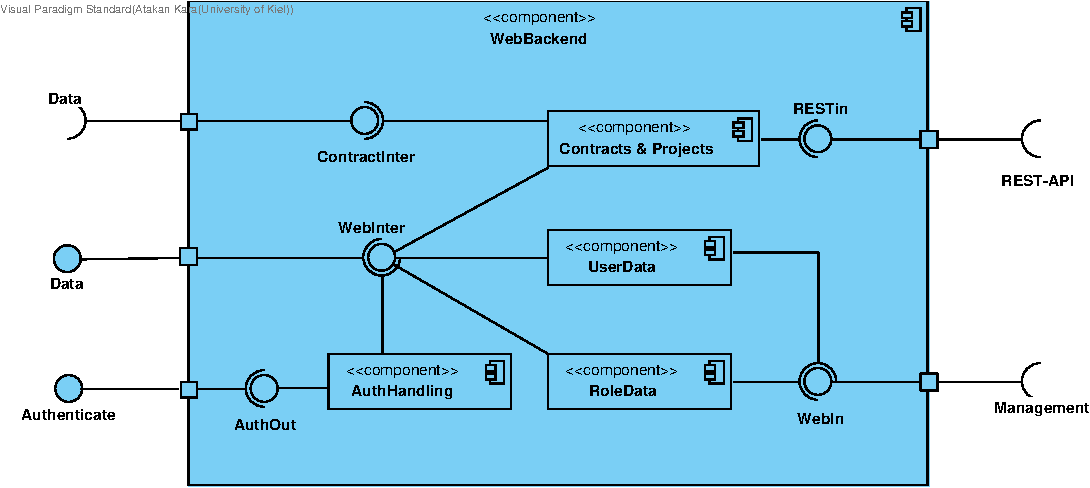
\includegraphics[width=16cm]{img/diagrams/cp_backend.pdf}	
	\caption{Komponentendiagramm - Backend}
	\label{fig:komponentendiagramm-backend}
\end{figure}

\clearpage

\begin{longtable}[h]{p{4cm} p{10.0cm}}
	\caption{Tabelle - Komponentendiagramm-Backend}
	\centering
	\label{tab:table_comp_backend}
	\endlastfoot
	\multicolumn{2}{r}{{Weitergeführt auf der folgenden Seite}} \\
	\endfoot
	\endhead
	\rowcolor[HTML]{C0C0C0} 
	\textbf{Komponente} & \textbf{Beschreibung} \\ 
	
	Authenticate & Gibt die Daten nach dem Authentifizierungsvorgang zurück. \\
	
	\rowcolor[HTML]{E7E7E7} 
	AuthHandling & Verwaltet den Authentifizierungsvorgang.  \\
	
	Contracts {\&} Projects & Speichert die Vertrags- und Projektdaten aus der REST-API. \\
	
	\rowcolor[HTML]{E7E7E7} 
	Data & Das eingehende Interface empfängt die Anfragen des \textbf{WebServers} für den Erhalt und die Veränderung bestimmter Vertrags- und Projektdaten. Das ausgehende Interface gibt, falls passende Berechtigungen bestehen, die abgefragten Daten, eine Bestätigung oder eine Fehlermeldung aus.  \\
	
	Management & Nimmt Daten vom \textbf{OrgAdmin} oder \textbf{SysAdmin} entgegen und übergibt diese über das Interface \textbf{WebIn} intern der \textbf{RoleData} und \textbf{UserDate}. \\
	
	\rowcolor[HTML]{E7E7E7} 
	REST-API & Fragt die Daten von der REST-API ab und übergibt diese über das Interface \textbf{RESTin} der Komponente \textbf{Contracts {\&} Projects}. \\
	
	RoleData & Speichert die vom \textbf{OrgAdmin} erstellten Rollen und deren Berechtigungen ab. \\
	
	\rowcolor[HTML]{E7E7E7} 
	UserData & Speichert die Nutzerdaten, so wie Name, Passwort und assoziierte Rolle.
\end{longtable}

\clearpage

\section{Web}

\begin{figure}[H]
	\centering
	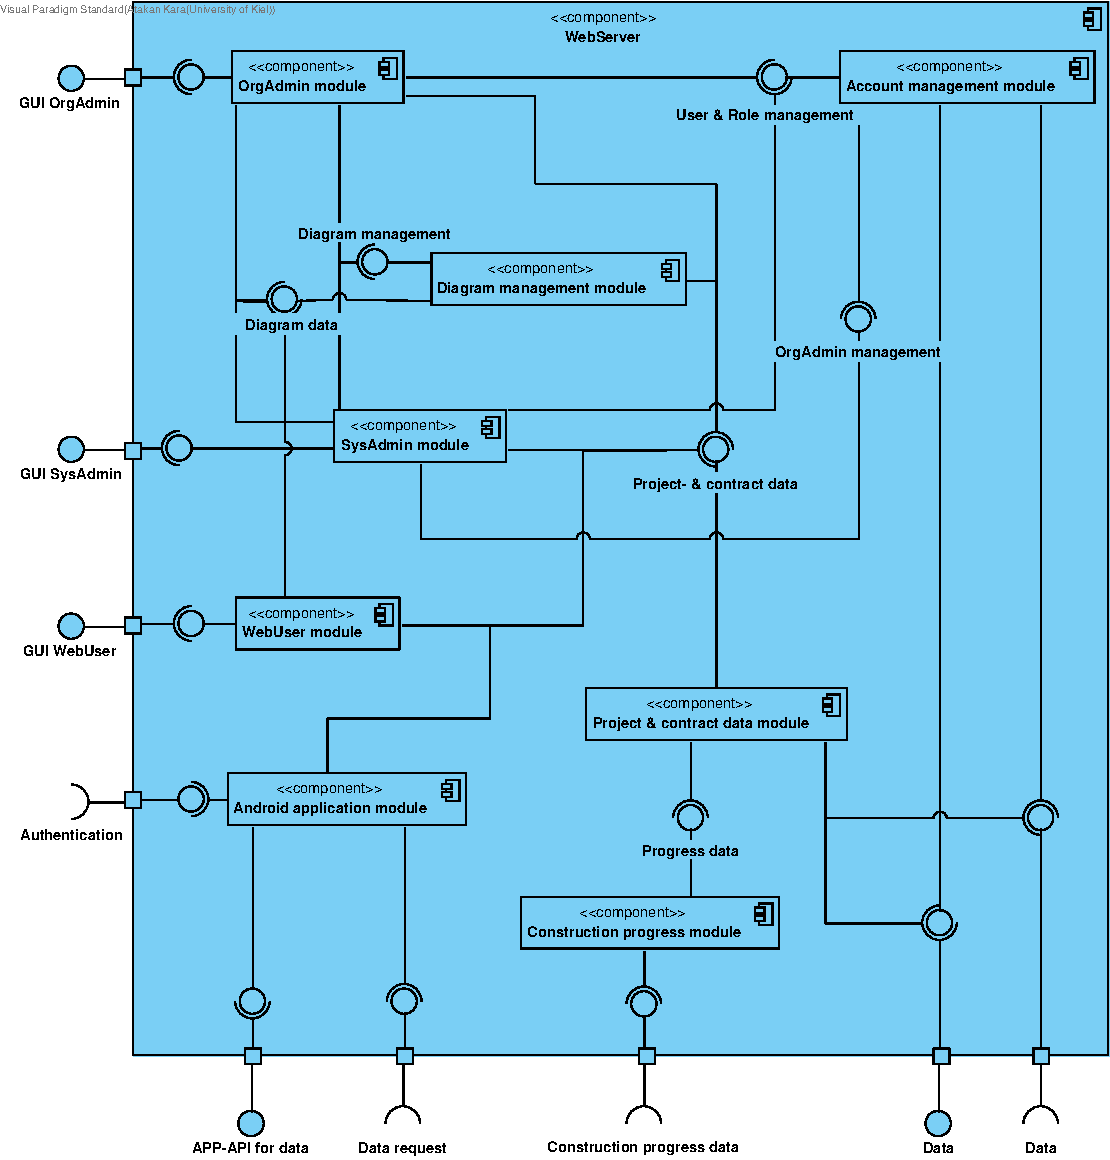
\includegraphics[width=16cm]{img/diagrams/Component-WebServer.pdf}	
	\caption{Komponentendiagramm - WebServer}
	\label{fig:komponentendiagramm-webserver}
\end{figure}

\clearpage

\begin{longtable}[h]{p{4cm} p{10.0cm}}
	\caption{Tabelle - Komponentendiagramm-WebServer}
	\centering
	\label{tab:table_comp_webserver}
	\endlastfoot
	\multicolumn{2}{r}{{Weitergeführt auf der folgenden Seite}} \\
	\endfoot
	\endhead
	\rowcolor[HTML]{C0C0C0} 
	\textbf{Komponente} & \textbf{Beschreibung} \\
	
	Account management & Modul zur Anzeige und graphischen Verwaltung von \textbf{OrgAdmins}, \textbf{WebUser} und deren Rollen. \\
	
	\rowcolor[HTML]{E7E7E7} 
	Android application module & Modul zur Verwaltung der \textbf{App}. Leitet Authentifizierungs- und Datenanfragen weiter. \\
	
	APP-API for data & Schnittstelle zur Datenübermittlung zur \textbf{App}. \\
	
	\rowcolor[HTML]{E7E7E7} 
	Authentication & Schnittstelle zur Weiterleitung der Authentifizierungsanfrage des \textbf{AppUser}s zum \textbf{Backend}. \\
	
	Construction progress & Modul zur Übermittlung von Baufortschrittsdaten. \\
	
	\rowcolor[HTML]{E7E7E7} 
	Construction progress data & Eingang der Baufortschrittsdaten der App, wie z.B. Fotos und deren Beschreibungen. \\
	
	Data & Ein- und Ausgang von Projekt-, Vertrags-, und Kontodaten zum und vom \textbf{Backend}. \\
	
	\rowcolor[HTML]{E7E7E7} 
	Data request & Erhalt der Anfragen zur Datenübermittlung von der \textbf{App}. \\
	
	Diagram management module & Modul zur Verwaltung und Anzeige von Diagrammen. \\
	
	\rowcolor[HTML]{E7E7E7} 
	Project {\&} contract data module & Modul zur Verwaltung und Weiterleitung von Projekt- und Vertragsdaten. \\
	
	GUI OrgAdmin & Eingehende Daten und graphische Nutzeroberfläche des \textbf{OrgAdmin}s. Dieser muss eingeloggt sein. \\
	
	\rowcolor[HTML]{E7E7E7} 
	GUI SysAdmin & Eingehende Daten und graphische Nutzeroberfläche des \textbf{SysAdmin}s. Dieser muss eingeloggt sein. \\
	
	GUI WebUser & Eingehende Daten und graphische Nutzeroberfläche des \textbf{WebUser}s. Dieser muss eingeloggt sein. \\
	
	\rowcolor[HTML]{E7E7E7} 
	OrgAdmin & Vereinigt die Interaktionsmöglichkeiten des \textbf{OrgAdmin} in einem zentralen Modul. \\
	
	SysAdmin & Vereinigt die Interaktionsmöglichkeiten des \textbf{SysAdmin} in einem zentralen Modul. \\
	
	\rowcolor[HTML]{E7E7E7} 
	WebUser & Vereinigt die Interaktionsmöglichkeiten des \textbf{AppUser} in einem zentralen Modul.
\end{longtable}

\clearpage

\section{App}

\begin{figure}[H]
	\centering
	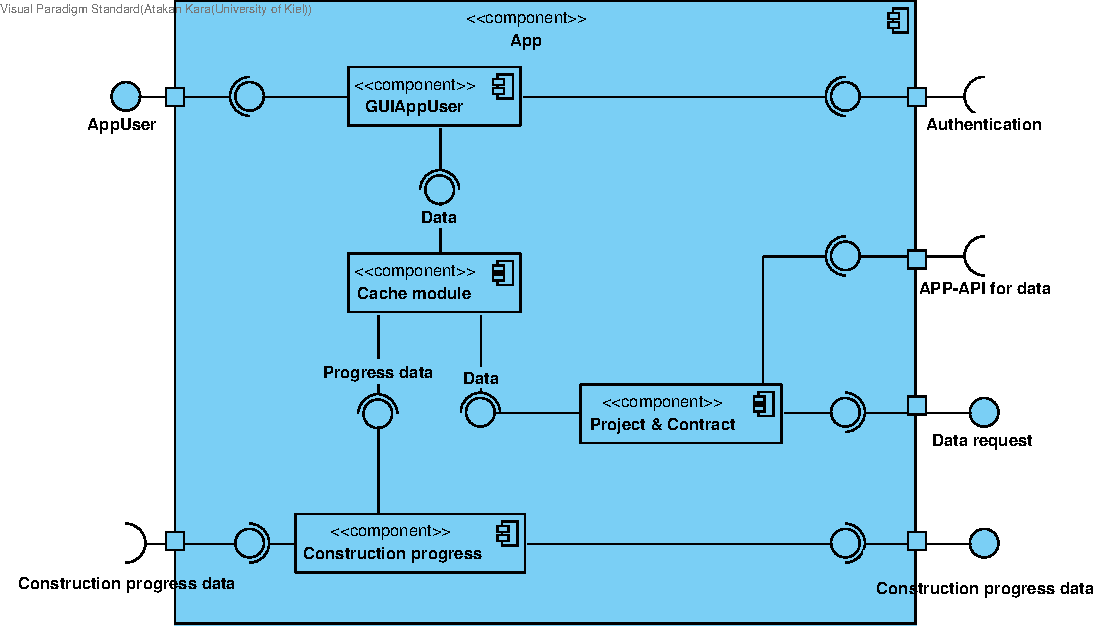
\includegraphics[width=16cm]{img/diagrams/Component-App.pdf}
	\caption{Komponentendiagramm - App}
	\label{fig:komponentendiagramm-app}
\end{figure}


\begin{longtable}[h]{p{4cm} p{10.0cm}}
	\caption{Tabelle - Komponentendiagramm-App}
	\centering
	\label{tab:table_comp_app}
	\endlastfoot
	\multicolumn{2}{r}{{Weitergeführt auf der folgenden Seite}} \\
	\endfoot
	\endhead
	\rowcolor[HTML]{C0C0C0} 
	\textbf{Komponente} & \textbf{Beschreibung} \\ 
	
	AppUser & Schnittstelle für den Nutzer der Applikation, um alle möglichen Daten einzusehen. \\
	
	\rowcolor[HTML]{E7E7E7} 
	APP-API for data & Schnittstelle zum Erhalt von Projekt- und Vertragsdaten vom \textbf{WebServer}. \\
	
	Authentication & Übermittelt notwendige Daten zum \textbf{WebServer} zur Authentifizierung des \textbf{AppUser}. \\
	
	\rowcolor[HTML]{E7E7E7} 
	Cache module & Dient der Zwischenspeicherung der Projekt- und Vertragsdaten sowie des Baufortschritts. \\
	
	Construction progress & Verwaltet den Baufortschritt. \\
	
	\rowcolor[HTML]{E7E7E7} 
	Construction progress data & Das eingehende Interface erhält Daten zum Baufortschritt, wie z.B. Fotos und deren Beschreibungen. Diese fügt der \textbf{AppUser} hinzu. Das ausgehende Interface hingegen übermittelt diese an den \textbf{WebServer}. \\
	
	Data request & Schnittstelle zur Anfrageübermittlung zum \textbf{WebServer}. \\
	
	\rowcolor[HTML]{E7E7E7} 
	GUIAppUser & Modul zur Darstellung der graphischen Nutzeroberfläche der \textbf{App}. \\
	
	Project {\&} Contract & Verwaltet die Projekt- und Vertragsdaten.
\end{longtable}

\clearpage
	
	\chapter{Verteilungsdiagramm}\label{chp:verteilungsdiagramm}
	\thispagestyle{fancy}
	\begin{figure}[h]
	\centering
	\missingfigure{Verteilungsdiagramm}		
	\caption{Verteilungsdiagramm}
	\label{fig:verteilungsdiagramm}
\end{figure}

\begin{tcolorbox}
	Das zukünftige Deployment des Systems wird mittels einem Verteilungsdiagramm modelliert.
	Weiterhin sollten wichtige oder eventuell undeutliche Zusammenhänge (z.B. warum Schnittstelle X genutzt wird) in einem Fließtext beschrieben werden.
\end{tcolorbox}
		
	\chapter{Klassendiagramme}\label{chp:klassendiagramme}
	\thispagestyle{fancy}
	%\begin{tcolorbox}
%Teilt eure Klassendiagramme bitte auf und baut \textbf{kein} einzelnes riesiges Diagramm.
%Getter und Setter Methoden müssen hier nicht modelliert werden.
%Sie sollten aber der klassischen Namenskonvention folgen, um die Nutzung in Sequenzdiagrammen zu ermöglichen.
%\\\\
%Auf jedes Diagramm folgt eine Tabelle, in der die Aufgabe \textbf{jeder} Klasse beschrieben wird.
%\end{tcolorbox}

\section{Backend}

\subsection{Backend Datenmodell}

\begin{figure}[H]
	\centering
	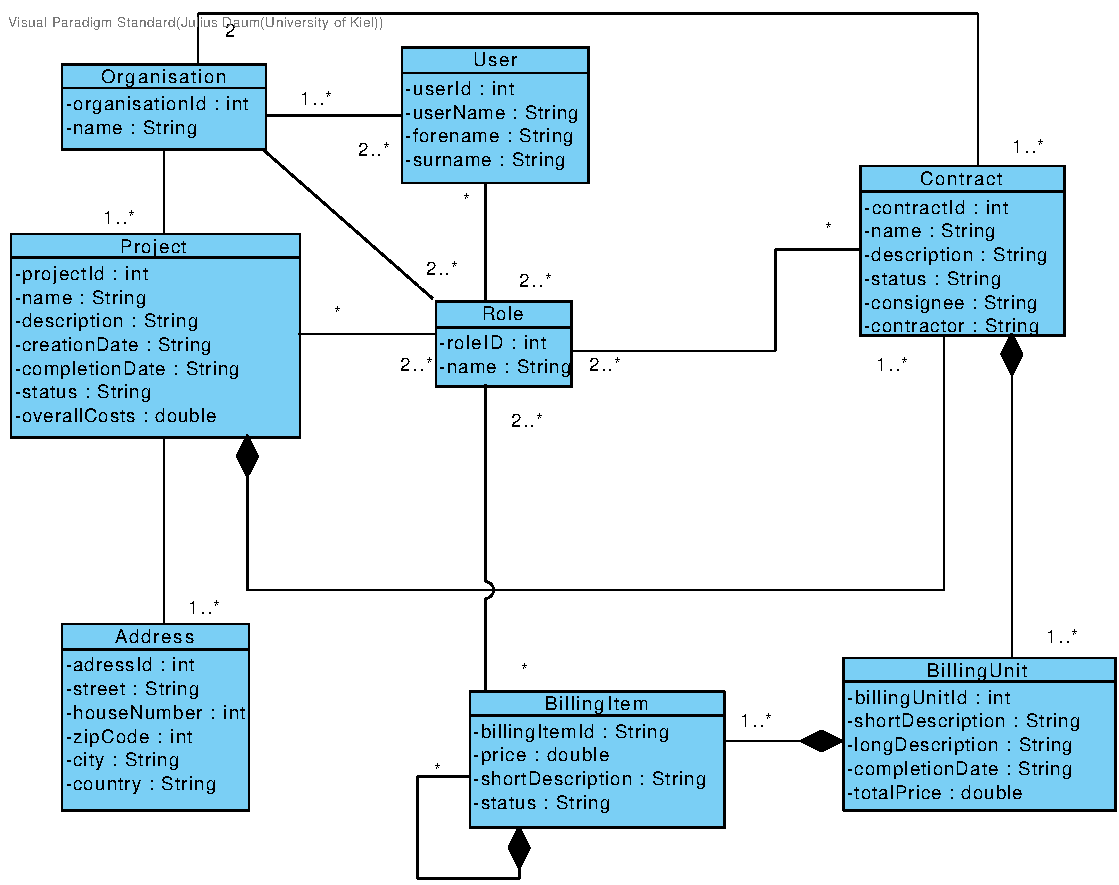
\includegraphics[width=\linewidth]{img/diagrams/class-diagram-backend.pdf}
	\caption{Klassendiagramm - Backend}
	\label{fig:klassendiagramm-backend}
\end{figure}

\clearpage

\noindent
Dieses Klassendiagramm enthält die Entitäten der Datenbank, jede Klasse entspricht einer Entität. \\
Die Klasse Role besitzt zu den Klassen BillingItem, Contract, User, Organisation und Project min. 2 Rollen. \\
Dies ist damit zu begründen, dass der SysAdmin Teil jeder Organisation ist und somit alle Projekte, User, Verträge und Leistungspositionen einsehen kann.
Zusätzlich existiert zu jeder Organisation min. ein OrgAdmin, der ebenfalls auf alle Verträge, Projekte und Leistungspositionen zugreifen kann.
 
\begin{longtable}[h]{p{5.3cm} p{8.7cm}}
	\caption{Klassenbeschreibung - Backend}
	\label{table:klassenbeschreibung-backend}
    \endlastfoot
	\multicolumn{2}{r}{{Weitergeführt auf der folgenden Seite}} \\
	\endfoot
	\endhead
	\rowcolor[HTML]{C0C0C0} 
	\textbf{Klassenname} & \textbf{Aufgabe} \\
    
	Address & Die Adresse des Projektes. \\
	
	\rowcolor[HTML]{E7E7E7} 
	BillingItem & Die Leistungspositionen eines Vertrages. \\
	
	BillingUnit & Eine Gruppierung von Leistungspositionen. \\
	
	\rowcolor[HTML]{E7E7E7} 
	Contract & Ein Vertrag, welcher zwischen zwei Parteien geschlossen wird. \\
	
	Organisation & Eine Gruppierung von Usern. \\
	
	\rowcolor[HTML]{E7E7E7} 
	Project & Ein Projekt min. einer Organisation, welches mehrere Verträge enhalten kann. \\
	
	Role & Nutzerrollen mit verschiedenen Rechten. Verwaltbar vom OrgAdmin. \\

	\rowcolor[HTML]{E7E7E7}
	User & Mitarbeiter min. einer Organisation.
\end{longtable}

\subsection{Backend Datenverarbeitung}

\begin{figure}[H]
	\centering
	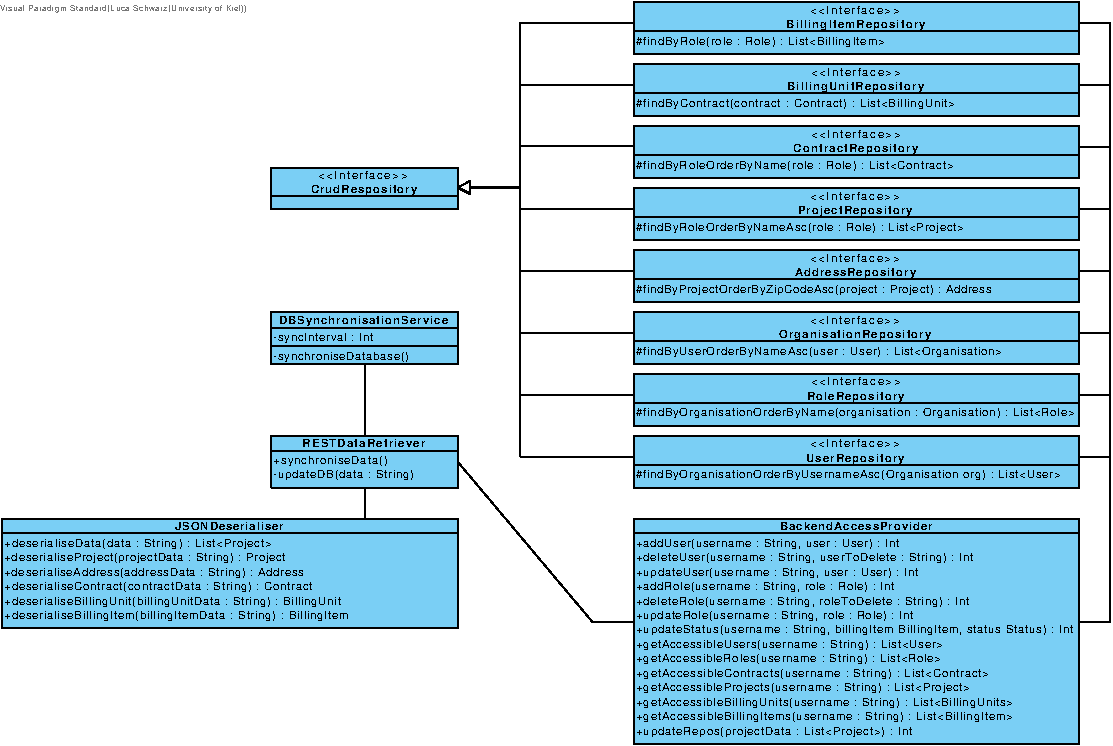
\includegraphics[width=\linewidth]{img/diagrams/Backend.pdf}
	\caption{Klassendiagramm - Backend - Datenverarbeitung}
	\label{fig:klassendiagramm-backend-data}
\end{figure}

\clearpage

\begin{center}
\begin{longtable}[h]{p{5cm} p{9cm}}
	\caption{Klassenbeschreibung - Backend - Datenverarbeitung}
	\label{table:klassenbeschreibung-backend-data}
	\endlastfoot
	\multicolumn{2}{r}{{Weitergeführt auf der folgenden Seite}} \\
	\endfoot
	\endhead
	\rowcolor[HTML]{C0C0C0} 
	\textbf{Klassenname} & \textbf{Aufgabe} \\
    CrudRepository & Teil des Spring Frameworks. Wird hier genutzt, um die Datenbank in From von erbenden Repositories darzustellen \\
	\rowcolor[HTML]{E7E7E7} 
	*Repository & Verwaltet die jeweilige Datenmodellklasse. Bietet spezielle Zugriffsfunktionen für eine einfachere Nutzung \\
	BackendAccessProvider & Bietet die eigentliche Funktionalität des Backends innerhalb der Server-Applikation an. Über diese Klasse wird der gesicherte Zugriff auf die gespeicherten Daten sichergestellt und die 
    einzelnen DatenRepositories werden vor dem Nutzer verborgen. Alle Methoden verlangen einen Nutzernamen als Parameter, um festzustellen welche Daten tatsächlch zurückgegeben werden dürfen. Dafür werden intern die Rollen verwendet.
    So soll ein Nutzer z.Bsp. nur Zugriff auf Verträge bekommen für welche er über eine entsprechende Rolle verfügt. Ansonsten werden leere Listen und auch Fehlercode zurückgegeben, welche dann z.Bsp. vom Frontend
    entsprechen verarbeitet werden können. Die Controller-Klassen des Frontends haben demnach Zugriff auf den BackendAccessProvider. \\
	\rowcolor[HTML]{E7E7E7} 
	DBSynchronisationService & Dienst, welcher die Aufgabe hat nach einer gewissen verschrittenen Zeit eine Synchronisation der Datenbeank mit der von adesso zu veranlassen. Die Eigentliche Synchronisation wird
    durch die Klasse RESTDataSynchroniser durchgeführt. \\
    RESTDataRetriever & Hat zur Aufgabe die Daten über die REST-API von adesso abzufragen und folgend die Daten zu deserialisieren. Die so erhaltenen Klassen werden abschließend in die Datenbank eingepflegt. \\
	\rowcolor[HTML]{E7E7E7} 
    JSONDeserialiser & Deserialisiert JSON-Strings zu den entsprechenden Modellklassen. Dies wird dann genutzt, wenn die über die REST-API von adesso Daten abgefragt werden. \\
\end{longtable}
\end{center}

\clearpage

\section{Web}

\begin{figure}[h]
	\centering
	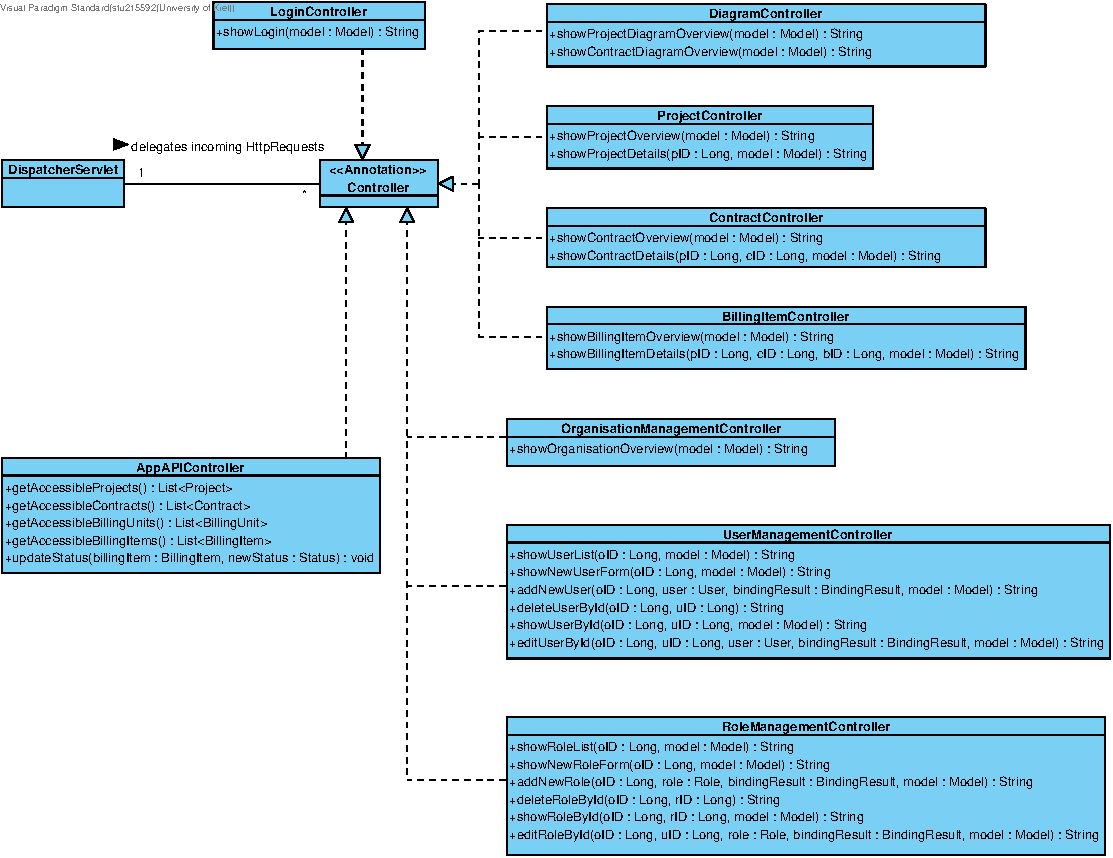
\includegraphics[width=\linewidth]{img/diagrams/Frontend Classes.pdf}
	\caption{Klassendiagramm - Frontend Web}
	\label{fig:klassendiagramm-web}
\end{figure}

\noindent
Klassen, deren Name mit ''Controller'' aufhört, verarbeiten HTTP Requests zu bestimmten Pfaden.
Die zu verarbeitenden Pfade sind pro Gebiet in einem jeweiligen Controller gruppiert.
In der folgenden Tabelle werden für Controller unter ''Aufgabe'' die zu verarbeitenden Pfade sowie die Bedeutung der dazugehörigen Seite aufgeführt.
Die Identifikationsnummern oID (Organisation), diaID (Diagramm), pID (Projekt), cID (Vertrag) und bID (Leistungsposition) sind in manche Pfade direkt integriert.\\

\begin{longtable}[h]{p{5.3cm} p{8.7cm}}
	\caption{Klassenbeschreibung - Frontend Web}
	\label{table:klassenbeschreibung-web}
	\endlastfoot
	\multicolumn{2}{r}{{Weitergeführt auf der folgenden Seite}} \\
	\endfoot
	\endhead
	\rowcolor[HTML]{C0C0C0} 
	\textbf{Klassenname} & \textbf{Aufgabe} \\
    
	DispatcherServlet & Teil des Spring Frameworks, leitet die HTTP Requests an den jeweils zuständigen Controller weiter \\
	
	\rowcolor[HTML]{E7E7E7} 
	LoginController & /login $\rightarrow$ Login-Seite \\
	
	OrganisationManagementController & /organisation\_overview $\rightarrow$ Management von Organisationen und deren OrgAdmins, nur der SysAdmin hat hierauf Zugriff \\
	
	\rowcolor[HTML]{E7E7E7} 
	UserManagementController & /organisation/\{oID\}/user\_management $\rightarrow$ Management der WebUser einer Organisation \newline\newline
	/organisation/\{oID\}/user\_management/user\_new $\rightarrow$ Hinzufügen eines WebUsers zu einer Organisation \newline\newline
	/organisation/\{oID\}/user\_management/user/\{uID\}/user\_edit $\rightarrow$ Bearbeiten eines WebUsers einer Organisation \\
	
	RoleManagementController & /organisation/\{oID\}/role\_management $\rightarrow$ Management der Rollen einer Organisation \newline\newline
	/organisation/\{oID\}/role\_management/role\_new $\rightarrow$ Hinzufügen einer Rolle zu einer Organisation \newline\newline
	/organisation/\{oID\}/role\_management/role/\{rID\}/role\_edit $\rightarrow$ Bearbeiten einer Rolle einer Organisation \\
	
	\rowcolor[HTML]{E7E7E7} 
	ProjectController & /project\_overview $\rightarrow$ Zeigt alle Projekte an, für welche der WebUser die nötigen Berechtigungen hat \newline\newline
	/project/\{pID\}/show $\rightarrow$ Zeigt die Verträge des Projekts an, für welche der WebUser die nötigen Berechtigungen hat \\
	
	ContractController & /contract\_overview $\rightarrow$ Zeigt alle Verträge an, für welche der WebUser die nötigen Berechtigungen hat \newline\newline
	/project/\{pID\}/contract/\{cID\}/show $\rightarrow$ Zeigt die Leistungspositionen des Vertrags an, für welche der WebUser die nötigen Berechtigungen hat \\
	
	\rowcolor[HTML]{E7E7E7} 
	BillingItemController & /billing\_item\_overview $\rightarrow$ Zeigt alle Leistungspositionen an, für welche der WebUser die nötigen Berechtigungen hat \newline\newline
	/project/\{pID\}/contract/\{cID\}/billing\_item/\{bID\}/show $\rightarrow$ Zeigt Details zur Leistungsposition an, falls der WebUser die nötigen Berechtigungen hat \\
	
	DiagramController & /project\_diagram\_overview $\rightarrow$ Zeigt alle Diagramme zu Projekten an, für welche der WebUser die nötigen Berechtigungen hat \newline\newline
	/contract\_diagram\_overview $\rightarrow$ Zeigt alle Diagramme zu Verträgen an, für welche der WebUser die nötigen Berechtigungen hat
\end{longtable}

\clearpage

\section{App}

\begin{figure}[h]
	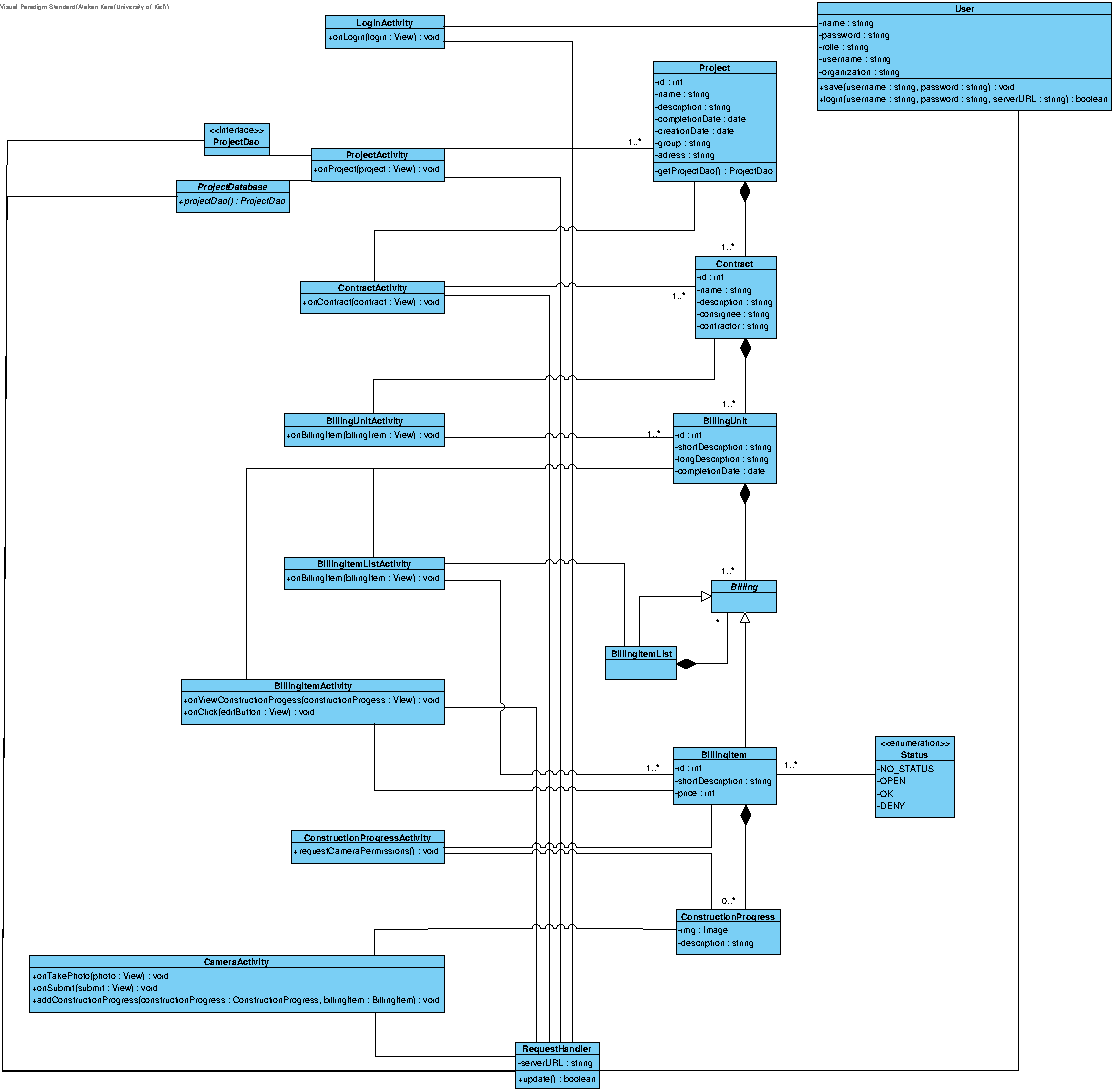
\includegraphics[width=16cm]{img/diagrams/Classdiagram-App.pdf}
	\caption{Klassendiagramm - App}
	\label{fig:klassendiagramm-a}
\end{figure}

\clearpage

\begin{table}[h]
	\centering
	\begin{tabularx}{\textwidth}{X X}
		\rowcolor[HTML]{C0C0C0} 
		\textbf{Klassenname} & \textbf{Aufgabe} \\
		Project & Bauplan eines Projektes mit den jeweiligen Attributen.\\
		\rowcolor[HTML]{E7E7E7} 
		Contract & Bauplan eines Vertrages mit den jeweiligen Attributen. \\
		BillingItem & Bauplan einer Leistungsposition mit den jeweiligen Attributen. \\
		\rowcolor[HTML]{E7E7E7} 
		ConstructionProgress & Bauplan einer Baufortschritts-Klasse mit den jeweiligen Attributen. \\
		LoginActivity & Verwaltung des Login-Bildschirms. \\
		\rowcolor[HTML]{E7E7E7} 
		ProjectActivity & Verwaltung des Projekt-Bildschirms. \\
		ContractActivity & Verwaltung des Vertags-Bildschirms. \\
		\rowcolor[HTML]{E7E7E7} 
		BillingItem & Verwaltung des Leistungspositions-Bildschirms. \\
		ConstructionProgressActivity & Verwaltung des Baufortschritts-Bildschirms. \\
		\rowcolor[HTML]{E7E7E7} 
		RequestHandler & Verwaltung der Netzwerkanfragen aller Klassen. \\
		ProjectDao & Datenzugriffsobjekt mit Anfragen zur Interaktion mit der Projektdatenbank. \\
		\rowcolor[HTML]{E7E7E7} 
		ProjectDatabase & Room-Datenbank für Projekte. \\
		ContractDao & Datenzugriffsobjekt mit Anfragen zur Interaktion mit der Vertragsdatenbank. \\
		\rowcolor[HTML]{E7E7E7} 
		ContractDatabase & Room-Datenbank für Verträge. \\
		BillingItemDao & Datenzugriffsobjekt mit Anfragen zur Interaktion mit der Leistungspositionsdatenbank. \\
		\rowcolor[HTML]{E7E7E7} 
		BillingItemDatabase & Room-Datenbank für Leistungspositionen. \\
		ConstructionProgressDao & Datenzugriffsobjekt mit Anfragen zur Interaktion mit der Baufortschritsdatenbank. \\
		\rowcolor[HTML]{E7E7E7} 
		ConstructionProgressDatabase & Room-Datenbank für den Baufortschritt. \\
		Status & Enumeration des Typs Status.
	\end{tabularx}
	\caption{Klassenbeschreibung - App}
	\label{table:klassenbeschreibung-a}
\end{table}
	
	\chapter{Sequenzdiagramme}\label{chp:sequenzdiagramme}
	\thispagestyle{fancy}
	%\begin{figure}[h]
%	\centering
%	\missingfigure{Sequenzdiagramm}		
%	\caption{Sequenzdiagramm - A}
%	\label{fig:sequenz-a}
%\end{figure}


%\begin{tcolorbox}
%Das dynamische Verhalten des Systems wird mittels Sequenzdiagrammen modelliert.
%Hier müssen wahrscheinlich geräteübergreifende Aufrufe modelliert werden.
%Findet dafür eine geeignete Notation und nutzt diese durchgehend! 
%Achtet weiterhin darauf, dass die anderen Methoden im Klassendiagramm zu finden sind.
%Manche Sequenzen erfordern sicherlich eine kurze schriftliche Beschreibung.
%\end{tcolorbox}

\section{Backend}

\begin{figure}[h]
	\centering
	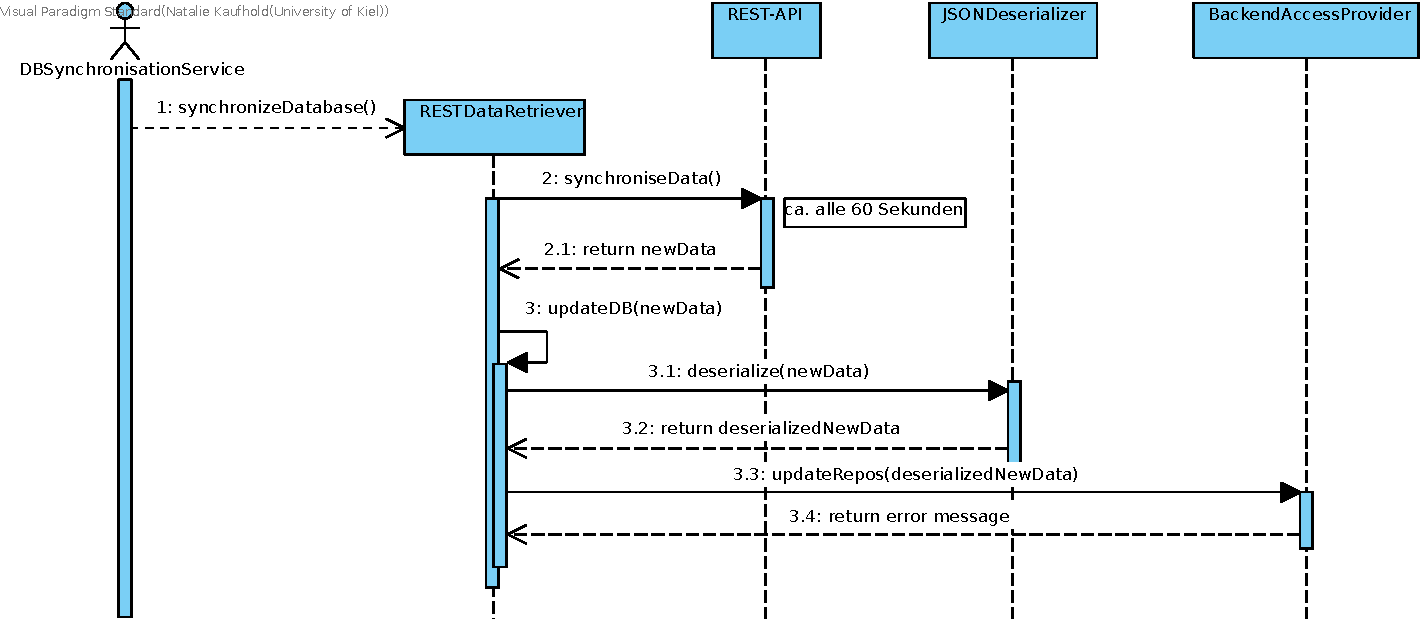
\includegraphics[width=\linewidth]{img/diagrams/RESThandling.pdf}	
	\caption{Sequenzdiagramm - A}
	\label{fig:sequenz-a}
\end{figure}

\noindent
Die neuen Daten werden von der REST-API als JSON zur Verfügung gestellt. Um die Daten aus der JSON-Datei in die Datenbank zu übertragen, muss  diese Datei in seine Einzelteile zerlegt werden: Dafür wird eine Instanz des JSONDeserializer verwendet, um die Daten etwa in eine Liste von Projekten zu konvertieren. Diese wird dann von einer Instanz des BackendAccessProviders in die Datenbank über die von Spring gestellten Repros übertragen.
Die Klasse REST-API wird vom Kunden gestellt und verwaltet. Darauf haben wir keinen Einfluss.

\clearpage

\section{App}
\begin{figure}[H]
	\centering
	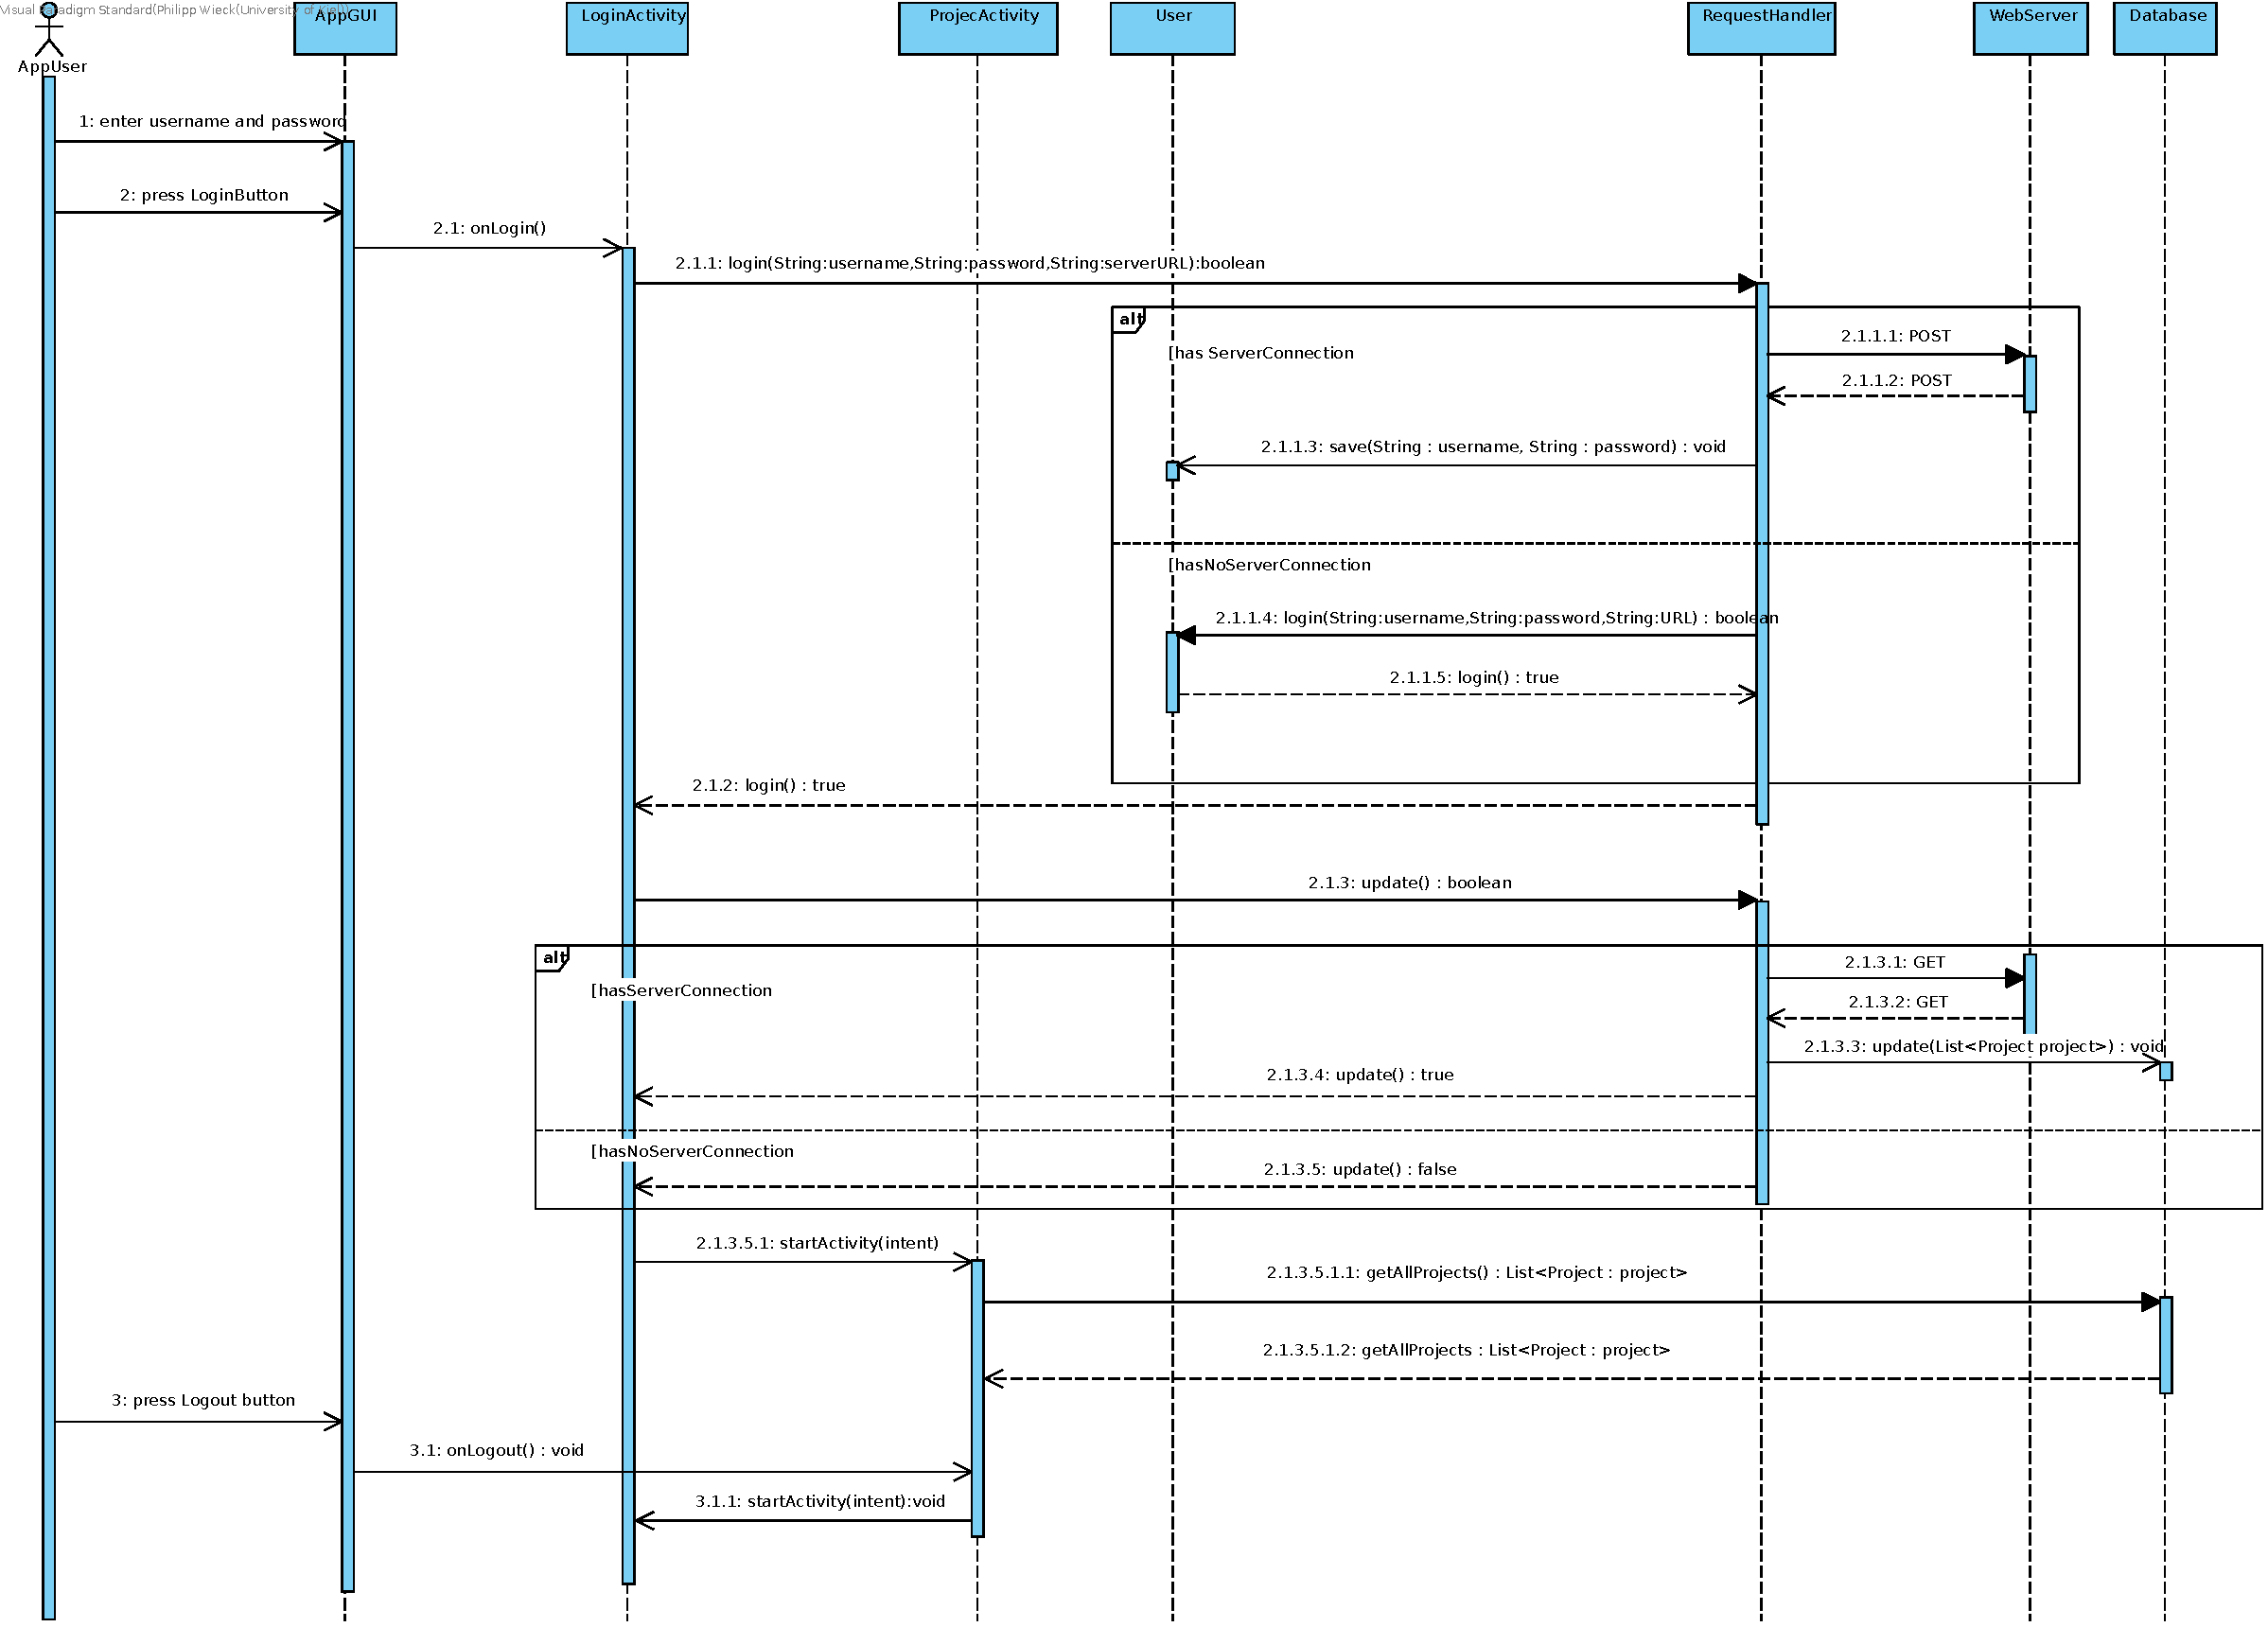
\includegraphics[width=\linewidth]{img/diagrams/App login, pull data, logout.pdf}		
	\caption{Login und Logout - App}
	\label{fig:sequenzdiagramm-app}
\end{figure}

\begin{figure}[H]
\centering
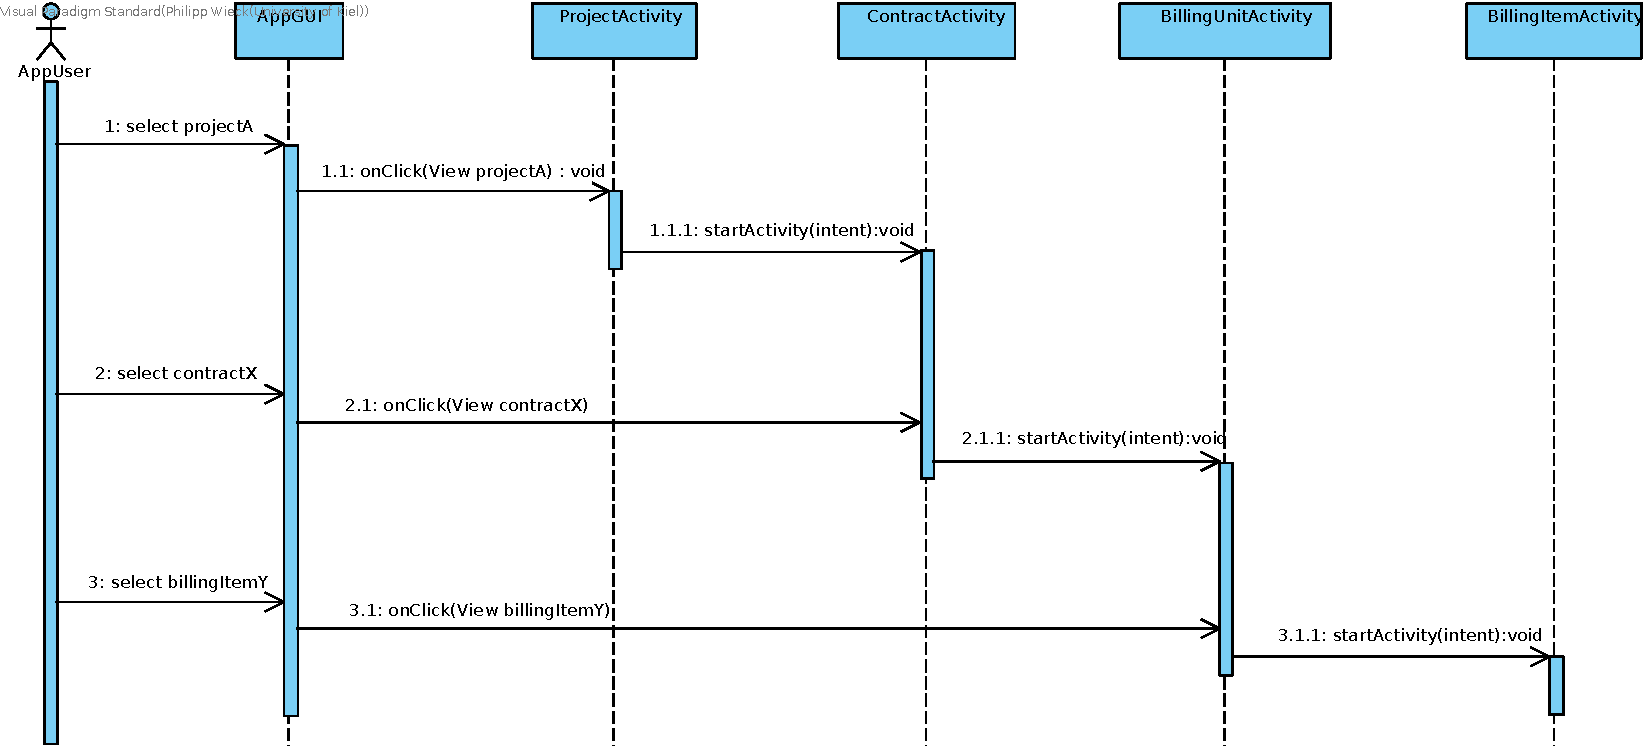
\includegraphics[width=\linewidth]{img/diagrams/Select BillingItem.pdf}		
\caption{Auswählen einer Leistungsposition - App}
\label{fig:sequenzdiagramm-app}
\end{figure}

\begin{figure}[H]
	\centering
	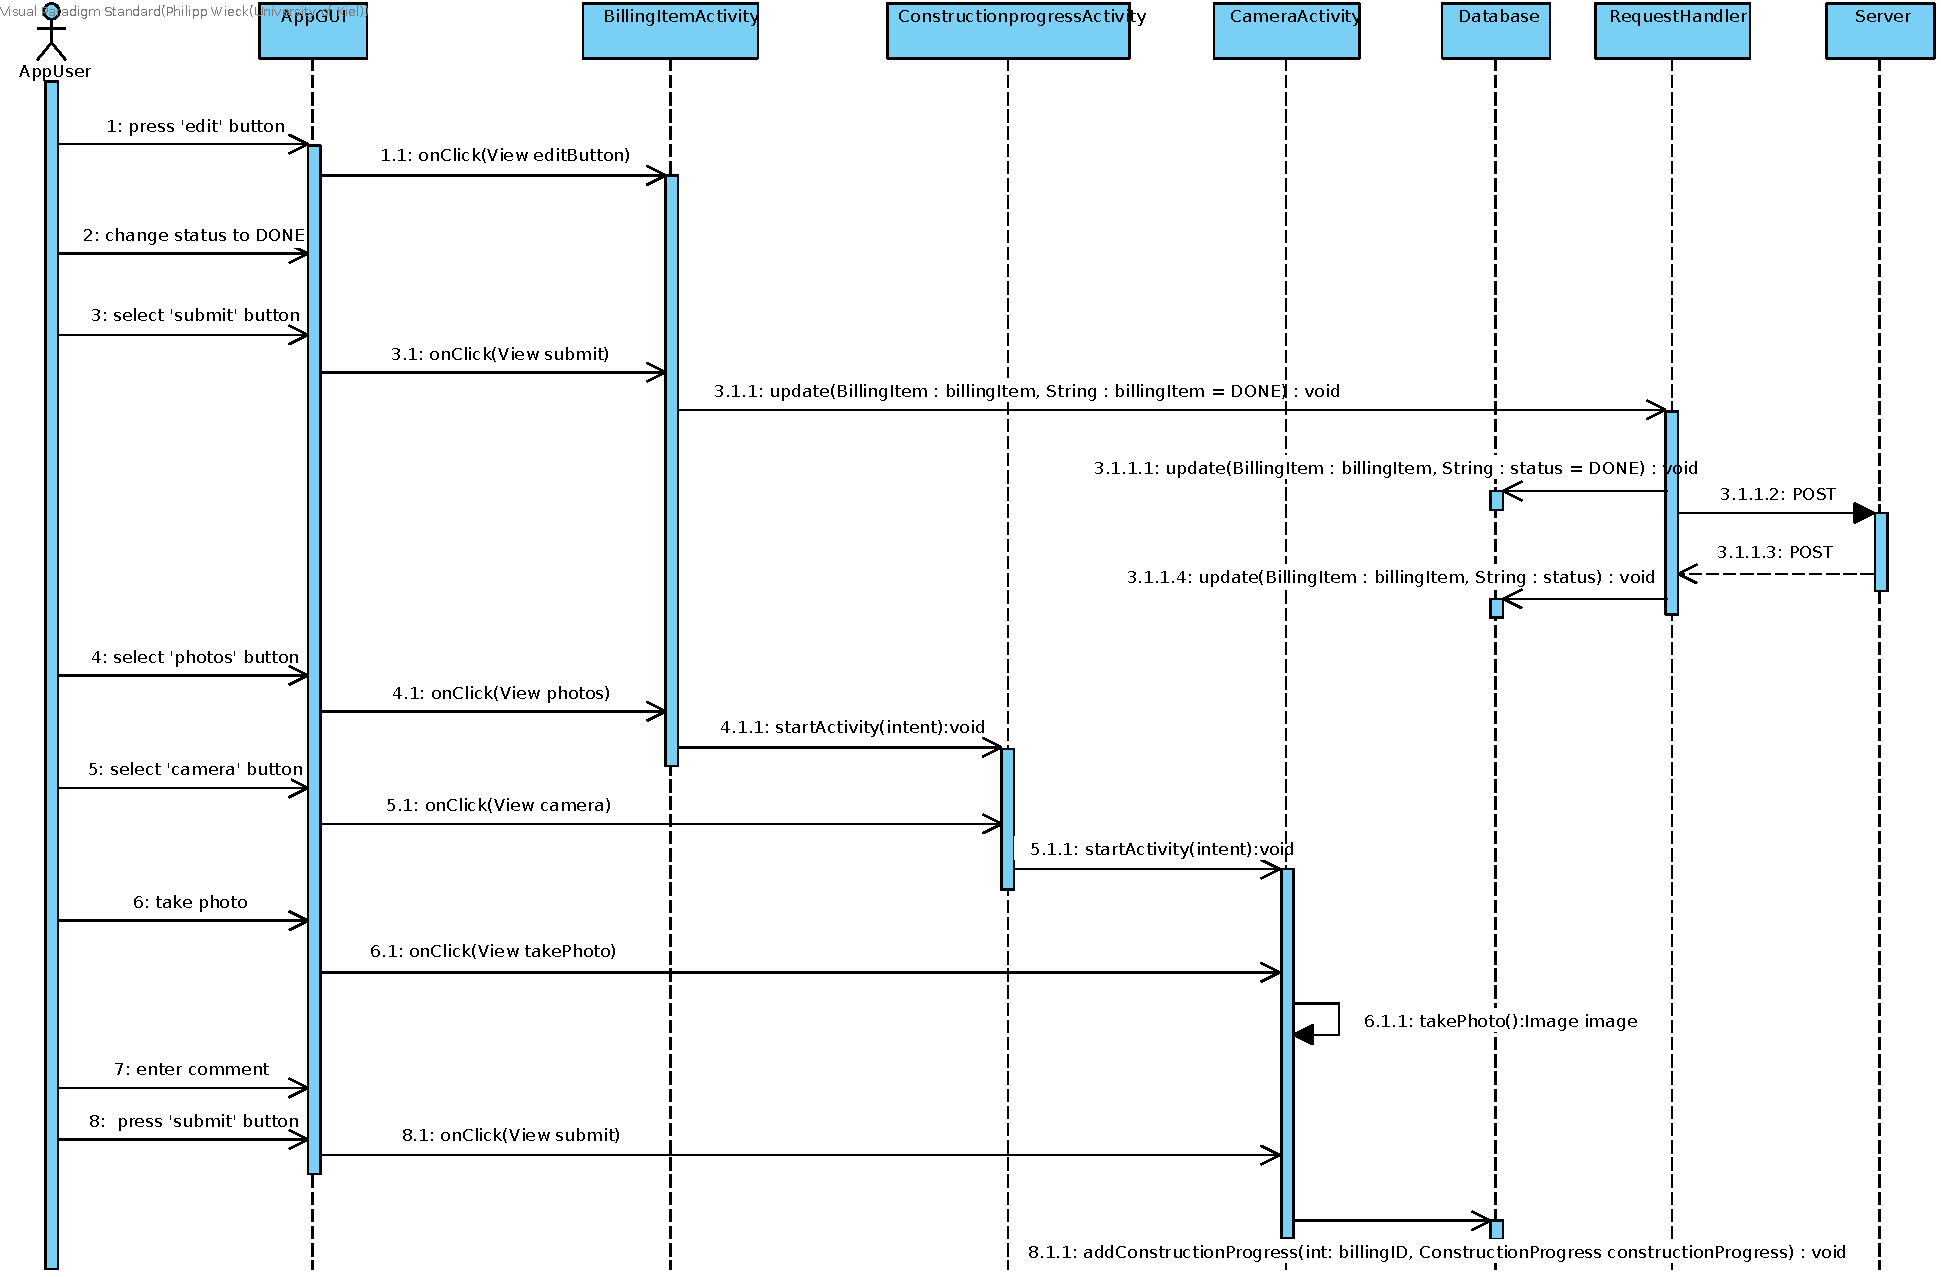
\includegraphics[width=\linewidth]{img/diagrams/change status, take photo.pdf}		
	\caption{Verändern des Status und Hinzufügen eines Fotos inkl. Kommentar - App}
	\label{fig:sequenzdiagramm-app}
\end{figure}
	
	\bibliography{references}
	\pagenumbering{gobble} % Nummerierung deaktivieren
	
\end{document}
